\normaltrue
\correctionfalse

%\UPSTIidClasse{12} % 11 sup, 12 spé
%\newcommand{\UPSTIidClasse}{12}

\exer{Mouvement T -- $\star$ \label{C1:05:01}}
\setcounter{numques}{0}
\UPSTIcompetence[2]{B2-14}
\UPSTIcompetence[2]{B2-15}
\UPSTIcompetence[2]{C1-05}
\index{Compétence B2-14}
\index{Compétence C1-05}
\index{Torseur des actions mécaniques transmissibles}
\index{Torseur d’une action mécanique extérieure}
\index{Principe fondamental de la statique}
\index{PFS}
\index{Mécanisme à 1 translation}
\ifcorrection
\else
\textbf{Pas de corrigé pour cet exercice.}
\fi

\ifprof
\else
Soit le mécanisme suivant. On note $\vect{AB}=\lambda(t)\vect{i_0}$. On note $m_1$ la masse du solide.
On note $G$ le centre d'inertie de \textbf{1} tel que $\vect{BG}=\ell \vect{j_1}$. La pesanteur est telle que $\vect{g}=-g\vect{i_0}$. Un vérin pneumatique positionné entre \textbf{1} et \textbf{0} permet de maintenir \textbf{1} en équilibre. 
On souhaite prendre en compte les frottements secs dans la liaison glissière.
%M et $\inertie{B}{1}=\matinertie{A_1}{B_1}{C_1}{-D_1}{0}{0}{\bas{1}}$.
\begin{center}
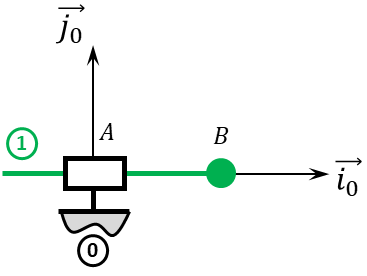
\includegraphics[width=.6\linewidth]{01_T_01}
\end{center}
\fi

\question{Réaliser le graphe d'analyse en faisant apparaître l'ensemble des actions mécaniques.}
\ifprof
\else
\fi

\question{Donner le torseur de chacune des actions mécaniques.}
\ifprof
\else
\fi


\question{Simplifier les torseurs dans l'hypothèse des problèmes plans.}
\ifprof
\else
\fi

\question{Proposer une démarche permettant de déterminer l'effort que doit développer le vérin pour maintenir \textbf{1} en équilibre.}
\ifprof
\else
\fi


\ifprof
\else
\begin{flushright}
\footnotesize{Corrigé  voir \ref{C1:05:01}.}
\end{flushright}%
\fi


